\documentclass{report}
\usepackage[spanish]{babel}
\usepackage[left=2.5cm, right=2.5cm, top=3cm, bottom=3cm]{geometry}
\usepackage{enumerate}
\usepackage{graphicx}
\usepackage{booktabs}
\usepackage{tabularx}
\usepackage{enumitem}
\usepackage{amsmath}
\usepackage{amsfonts}
\usepackage{float}
\usepackage{hyperref}   



\setlength{\parindent}{0pt}

\begin{document}

    \begin{titlepage}
        \centering
        {\bfseries\LARGE Facultad de Matemática y Computación \par}
        \vspace*{1cm}
        {\scshape\Large Ingeniería de Software \par}
        \vspace*{3cm}
        {\scshape\Huge Informe de Especificación de Requerimientos \par}
        \vspace*{1cm}
        {\LARGE \textbf{Tema: Gestión de campeonatos de béisbol} }
        \vfill
        {\bfseries\LARGE Integrantes: \par}
        {\Large Ariadna Vel\'azquez Rey  C311 \par} 
        {\Large L\'ia L\'opez Rosales  C312 \par} 
        {\Large Carlos Daniel Largacha Leal  C312 \par} 
        {\Large Gabriel Andr\'es Pla Lasa  C311 \par} 
        {\Large Raidel Miguel Cabellud Lizaso C311 \par} 
        \vfill
    \end{titlepage}

    \begin{center}
        \section*{Introducción}
    \end{center}

        \subsection*{Propósito del Documento}
        El propósito de este documento es definir y detallar los requerimientos del sistema de gestión de campeonatos de béisbol. Su objetivo principal es servir como una referencia clara y precisa para los desarrolladores, diseñadores y demás partes interesadas en el proyecto, asegurando que la aplicación cumpla con las necesidades de los usuarios. 

        Proporciona una visión integral del sistema, abarcando su alcance, funcionalidades, restricciones y requisitos técnicos. Además, establece las bases para futuras mejoras y mantenibilidad, garantizando una implementación eficiente y alineada con las expectativas del cliente y los usuarios finales.


        \subsection*{Alcance del Producto}

        Este proyecto tiene como objetivo el desarrollo de una aplicación web que facilite la gestión de los 
        campeonatos de béisbol. Su propósito principal es permitir a los usuarios consultar y analizar información 
        relevante de las series y los peloteros, proporcionando herramientas que soporten la toma de decisiones 
        basada en estadísticas detalladas y actualizadas. El sistema será accesible, eficiente y adaptado a las 
        necesidades de diversos usuarios, desde administradores hasta periodistas.


        \subsection*{Definiciones, acrónimos y abreviaturas}
        \textbf{PDF(Portable Document Format):} Es un formato de almacenamiento para documentos 
        digitales independientes de plataformas de software o hardware.

        \subsection*{Referencias}

        \subsection*{Resumen del resto del documento}
        El presente documento se estructura en varias secciones clave:

        \begin{itemize}
            \item \textbf{Descripción General:} Se proporciona una visión global del sistema, incluyendo su propósito, alcance y los actores involucrados.
            \item \textbf{Requerimientos Funcionales:} Se detallan las funciones esenciales del sistema.
            \item \textbf{Requerimientos No Funcionales:} Se especifican criterios como usabilidad, seguridad, escalabilidad y compatibilidad que el sistema debe cumplir.
            \item \textbf{Requerimientos de Entorno:} Se definen los aspectos técnicos necesarios para el correcto funcionamiento del software, incluyendo hardware, software y bases de datos.
            \item \textbf{Anexos:} Se incluyen diagramas y material adicional que complementan la especificación de requerimientos.
        \end{itemize}

    \newpage

    \begin{center}
        \section*{Descripción General}
    \end{center}

        \subsection*{Perspectiva del Producto}
        La aplicación web será una solución integral para la gestión y consulta de estadísticas en campeonatos de 
        béisbol. Estará diseñada para ofrecer:
        \begin{itemize}
            \item Acceso a estadísticas detalladas de series, equipos y jugadores.
            \item Generación de reportes personalizados.
            \item Funcionalidades diferenciadas según el rol del usuario (administrador, director técnico, 
            periodista/usuarios generales, etc.).
        \end{itemize}

        \subsection*{Funciones del Producto}
        
        \begin{enumerate}
        \item \textbf{Descripción de los Actores}

            \begin{itemize}
                \item \textbf{Administrador:} Responsable de gestionar los datos de series, equipos y jugadores, 
                además de configurar el sistema y generar reportes.
                \item \textbf{Director Técnico:} Encargado de gestionar las alineaciones de los equipos y consultar 
                estadísticas específicas.
                \item \textbf{Periodista/Usuario General:} Consulta las estadísticas y genera reportes basados en 
                los datos almacenados en el sistema.
            \end{itemize}

        \item \textbf{Casos de Uso del Sistema} (que se muestran ilustrados en la Figura 1)
            
            \subsubsection{Registrar datos en el sistema}
            \begin{itemize}
                \item \textbf{Actor:} Administrador
                \item \textbf{Descripción:} El administrador registra datos de series, equipos y jugadores mediante 
                formularios en la aplicación web.
            \end{itemize}

            \subsubsection{Gestionar alineaciones de equipos}
            \begin{itemize}
                \item \textbf{Actor:} Director Técnico y Administrador
                \item \textbf{Descripción:} Permite al director técnico modificar la posición de los jugadores en 
                la alineación inicial y realizar ajustes durante una serie.
            \end{itemize}

            \subsubsection{Consultar estadísticas de jugadores y equipos}
            \begin{itemize}
                \item \textbf{Actor:} Administrador, Director Técnico, Periodista/Usuario General
                \item \textbf{Descripción:} El sistema permite acceder a estadísticas detalladas, como promedios de 
                bateo, efectividad de los lanzadores y resultados de los equipos.
            \end{itemize}

            \subsubsection{Obtener reportes personalizados}
            \begin{itemize}
                \item \textbf{Actor:} Administrador, Director Técnico, Periodista/Usuario General
                \item \textbf{Descripción:} Genera reportes en formato PDF o gráficos que resumen el desempeño de 
                jugadores y equipos en una serie.
            \end{itemize}

            \subsubsection{Visualizar datos tabulares y gráficos}
            \begin{itemize}
                \item \textbf{Actor:} Administrador, Director Técnico, Periodista/Usuario General
                \item \textbf{Descripción:} Presentación visual de estadísticas mediante tablas y gráficos para un 
                análisis claro y rápido.
            \end{itemize}

            \subsubsection{Listar equipos por clasificación}
            \begin{itemize}
                \item \textbf{Actor:} Administrador, Director Técnico, Periodista/Usuario General
                \item \textbf{Descripción:} Permite obtener la clasificación de los equipos según los resultados de 
                cada serie.
            \end{itemize}

            \subsubsection{Modificar roles de usuarios}
            \begin{itemize}
                \item \textbf{Actor:} Administrador
                \item \textbf{Descripción:} El administrador puede asignar o modificar roles para los usuarios del 
                sistema.
            \end{itemize}

            \subsubsection{Exportar reportes a formato PDF}
            \begin{itemize}
                \item \textbf{Actor:} Administrador, Director Técnico, Periodista/Usuario General
                \item \textbf{Descripción:} Funcionalidad para guardar reportes generados en formato PDF, con 
                soporte para otros formatos adicionales.
            \end{itemize}

        \end{enumerate}


        \subsection*{Características de los usuarios}
        El sistema contará con diferentes perfiles de usuarios:
        \begin{itemize}
            \item \textbf{Administradores}: Control total del sistema, incluyendo la estructura de las series.
            \item \textbf{Directores Técnicos}: Gestión de alineaciones y rendimiento de los equipos.
            \item \textbf{Periodistas/Usuarios Generales}: Consulta de información general sobre los campeonatos. 
            Acceso a estadísticas y reportes para análisis independiente.
        \end{itemize}


        \subsection*{Restricciones generales}
        \begin{itemize}
            \item \textbf{Accesibilidad}: La aplicación será multiplataforma, garantizando su uso desde dispositivos 
            móviles y de escritorio.
            \item \textbf{Disponibilidad}: Asegurará el acceso continuo a la información para usuarios autorizados.
            \item \textbf{Tecnologías}: El desarrollo empleará Django como ORM, bajo una arquitectura hibrida de 
            N-Capas con Microkernel, siguiendo la metodología DIC.
            \item \textbf{Seguridad}: Se implementarán mecanismos para proteger la confidencialidad, integridad y 
            disponibilidad de los datos.
        \end{itemize}

        \subsection*{Dependencias y suposiciones}
        El software no estará sujeto a ningún SO pues se podrá acceder a él a través de cualquier navegador web que 
        el usuario posea.
        
        El lenguaje a utilizar será técnico referente al béisbol pues los usuarios están acontumbrados a él y es 
        necesario para un correcto manejo de los datos guardados.

    \newpage
    
    \begin{center}
        \section*{Requerimientos Específicos}
    \end{center}

    \vspace{0.5cm}

        \subsection*{Requerimientos Funcionales}
            \begin{enumerate}
                \item Registrar, editar, eliminar y listar datos por el administrador mediante formularios.
                \item Generar modelos tabulares y gráficos.
                \item Gestionar los roles de la base de datos que son los usuarios especiales (administrador), los 
                directores técnicos y los usuarios normales (periodista).
                \item Listar y filtrar según sus categorías definidas, nombres de equipos ganadores y directores 
                técnicos en series nacionales por temporada.
                \item Listar y filtrar según sus categorías definidas, nombres y posiciones de jugadores del equipo 
                "Todos Estrellas" y su efectividad por serie.
                \item Listar y filtrar según sus categorías definidas, series con mayor y menor cantidad de juegos 
                celebrados.
                \item Listar equipos en primer y último lugar por serie, clasificados por tipo y orden cronológico.
                \item Listar y filtrar según sus categorías definidas, total de juegos ganados por un lanzador y su 
                promedio de carreras limpias permitidas.
                \item Modificar posición de un jugador en la alineación inicial de un juego específico.
                \item Listar y filtrar según sus categorías definidas, estadísticas de un jugador.
                \item Exportar reportes a formato PDF con soporte para la agregación de otros formatos.
                \item Presentar diferentes vistas para los distintos tipos de roles.
                \item Generar formularios para ingresar los datos a la base de datos por parte del administrador 
                (distintos formularios para las distintas tablas de la base de datos).
                \item Tener un formulario para el director técnico que le permita crear, eliminar y listar los 
                cambios en  la alineación.
                \item Mostrar un formulario con opciones de filtrado y solicitudes para la generación de los reportes.
            \end{enumerate}

        \vspace{1cm}

        \subsection*{Requerimientos No Funcionales}

            \vspace{0.3cm}

            \subsubsection*{Usabilidad}
            \begin{itemize}
                \item Se espera que la interfaz sea capaz de mostrar gráficas.
                \item Se espera un sistema visual de filtrado para seleccionar qué datos mostrar en los reportes.
            \end{itemize}
        
            \subsubsection*{Seguridad}
            \begin{itemize}
                \item Todos los datos personales y críticos deben ser encriptados en tránsito y en almacenamiento.
                \item La autenticación y autorización deben ser seguras, permitiendo que solo los usuarios 
                autorizados tengan acceso a funcionalidades específicas.
            \end{itemize}
        
            \subsubsection*{Portabilidad y Compatibilidad}
            \begin{itemize}
                \item El diseño de la interfaz se espera que sea ajustable al tamaño de los distintos dispositivos 
                en los que puede abrirse el sitio web.
                \item Debe ser compatible con los navegadores más utilizados, asegurando que las interfaces web 
                sean responsivas y adaptativas.
            \end{itemize}
        
            \subsubsection*{Rendimiento}
            \begin{itemize}
                \item El sistema debe ser capaz de manejar múltiples solicitudes simultáneamente sin una degradación 
                significativa en el tiempo de respuesta.
            \end{itemize}
        
            \subsubsection*{Escalabilidad}
            \begin{itemize}
                \item La arquitectura debe permitir la escalabilidad horizontal y vertical. Esto significa que se 
                debe poder agregar más recursos (como servidores adicionales) para manejar un mayor número de 
                usuarios o datos sin necesidad de reestructurar significativamente el sistema.
            \end{itemize}
        
            \subsubsection*{Mantenibilidad}
            \begin{itemize}
                \item El sistema debe estar desarrollado con buenas prácticas de programación, como la documentación 
                adecuada (docstring) y código modular.
            \end{itemize}
        
            \subsubsection*{Extensibilidad}
            \begin{itemize}
                \item La arquitectura del sistema debe ser flexible para permitir la adición de nuevas funcionalidades 
                sin necesidad de grandes modificaciones en el código base.
            \end{itemize}
        
            \subsubsection*{Almacenamiento, importación y exportación de datos}
            \begin{itemize}
                \item El software deberá de almacenar todos los datos en una base de datos SQL.
                \item El software deberá ser capaz de convertir los reportes solicitados a documentos PDF.
            \end{itemize}

        \vspace{1cm}

        \subsection*{Requerimientos de Entorno}

            Para garantizar la ejecución del sistema, se deben cumplir las siguientes condiciones:

            \subsubsection{Hardware}
            \begin{itemize}
                \item Dispositivos capaces de ejecutar navegadores modernos y conexiones a internet estables.
            \end{itemize}
            
            \subsubsection{Software}
            \begin{itemize}
                \item Para la base de datos se ha de utilizar la tecnología PostgreSQL.
                \item En cuanto al backend de la aplicación web, este de desarrollará en Python con DjangoRest como 
                librería principal, omitiendo la función de admin que viene ya preparada.
                \item El frontend se realizará en JavaScript con el framework de React.
            \end{itemize}

    \newpage

    \section*{Anexos}

    \begin{figure}[H]
        \centering
        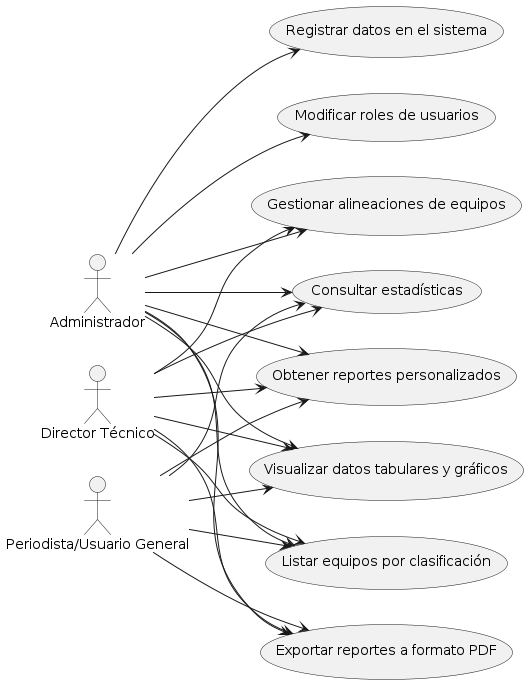
\includegraphics[scale=0.9,keepaspectratio]{caso_de_uso.png}
        \caption{Diagrama de casos de uso}
    \end{figure}


\end{document}